\chapter{Neural Networks}
In this chapter, we explore the oft spoken of neural networks. As we will come to see, neural networks are an extraordinarily flexible class of models used to solve a variety of different problem types. In fact, this flexibility is both what makes them so widely applicable and yet so difficult to use properly. We will explore the applications, underlying theory, and training schemes behind neural networks.

\section{Motivation}
Despite how seemingly popular neural networks have become recently, they aren't actually a novel technique. The first neural networks were described in the early 1940s, and the only reason they weren't put into practice shortly thereafter was the fact that we didn't yet have access to the large amounts of storage and compute that complex neural network require. Over the last two decades, and particularly with the advent of cloud computing, we now have more and more access to the cheap processing power and memory required to make neural networks a viable option for model building.

\subsection{Applications}
In the previous two chapters, we explored two broad problem types: classification and regression, and it's natural to wonder where neural networks fit in. The answer is that they are applicable to both. Neural networks are some of the most flexible models we will explore, and that flexibility extends to the types of problems they can be made to handle. Thus, the tasks that we've explored over the last two chapters, such as predicting heights in the regression case or object category in the classification case, can be performed by neural networks.

\subsection{Comparison to Other Methods}
Given that neural networks are flexible enough to be used as models for either regression or classification tasks, this means that every time you're faced with a problem that falls into one of these categories, you have a choice to make between the methods we've already covered or using a neural network. Before we've explored the specifics of neural networks, how can we discern at a high level when they will be a good choice for a specific problem?

One simple way to think about this is that if we never \textit{needed} to use neural networks, we probably wouldn't. In other words, if a problem can be solved effectively by one of the techniques we've already described for regression or classification (such as linear regression, discriminant functions, etc.), we would prefer to use those. The reason is that neural networks are often more memory and processor intensive than these other techniques, and they are much more complex to train and debug.

The flip side of this is that hard problems are often too complex, too ill-specified, or too poorly understood to use a simple regression or classification technique. Indeed, even if you eventually think you will need to use a neural network to solve a given problem, it makes sense to try a simple technique first both to get a baseline of performance and because it may just happen to be good enough.

What is so special about neural networks that they can solve problems that the other techniques we've explored may not be able to? And why are they so expensive? Those are the questions we turn to next.

\subsection{Strengths and Weaknesses}
For problems that fall into the category of regression or classification, we've already discussed the utility of basis functions. Sometimes, a problem that is intractable with our raw input data will be readily solvable with basis-transformed data. We often select these basis changes using expert knowledge. For example, if we were working with a data set that related to chemical information, and there were certain equations that a chemist told us to be important for the particular problem we were trying to solve, we might include a variety of the transformations that are present in those equations.

However, imagine now that we have a data set with no accompanying expert information. More often than not, complex problem domains don't come with a useful set of suggested transformations. How do we find useful basis functions in these situations? This is exactly the strength of neural networks - they solve for the best basis for a data set!

Neural networks can be used to simultaneously solve for our model parameters and the best basis transformations. This makes them exceedingly flexible.

Unfortunately, this flexibility is also the weakness of neural nets: while it enables us to solve difficult problems, it also creates a host of other complications. Chief among these complications is the fact that neural networks require a lot of computation to train. This is a result of the effective model space being so large - to explore it all takes time and resources. Furthermore, this flexibilty can cause rather severe overfitting if we are not careful.

In summary, the strengths and weaknesses of neural networks stem from the same root cause: model flexibility. It will be our goal then to appropriately harness this property to create useful models.

\subsection{Universal Function Approximation}
The flexibility of neural networks is a well-established phenomenon. In fact, neural networks are what are known as \textit{universal function approximators}. This means that with a large enough network, it is possible to approximate any function. The proof of this is beyond the scope of this textbook, but it provides some context for why flexibility is one of the key attributes of neural networks.

\begin{mlcube}{Neural Networks}
As universal function approximators, neural networks can operate over discrete or continuous inputs. That being said, it's far more common for them to accept \textbf{continuous} inputs. We primarily use neural networks to solve regression or classification problems, which involve training on data sets with example inputs and outputs, making this a \textbf{supervised} technique. Finally, while there exist probabilistic extensions for neural networks, they primarily operate in the \textbf{non-probabilistic} setting.
\begin{center}
    \begin{tabular}{c|c|c}
    \textit{\textbf{Domain}} & \textit{\textbf{Training}} & \textit{\textbf{Probabilistic}} \\
    \hline
    Continuous & Supervised & No \\
    \end{tabular}
\end{center}
\end{mlcube}

\section{Feed Forward Networks}
The feed forward neural network is the most fundamental setup for a neural network. Most of the logic behind neural networks can be explained using a feed forward network, with additional features typically added to form more complex networks. We will explore this basic neural network structure first.

\subsection{Adaptive Basis Functions}
As we mentioned in the introduction, the strength of neural networks is that we can learn an effective basis for our problem domain at the same time as we train the parameters of our model. In fact, learning this basis becomes just another part of our parameter training. Let's make this notion of learning a basis more concrete.

Thinking back to our chapter on linear regression, we were training a model that made predictions using a functional form that looked like:
\begin{align*}
	y(\textbf{x}, \textbf{w}) = \textbf{w} \boldsymbol{\phi}^{T} = \sum_{d=1}^{D} w_{d} \boldsymbol{\phi}_{d}
\end{align*}
where $\boldsymbol{\phi} = \phi(\textbf{x})$, $\phi$ is the basis transformation function, and $D$ is the dimensionality of our data point.

Typically with this linear regression setup, we are training our model to optimize the parameters $\textbf{w}$. With neural networks this is no different - we still train to learn those parameters. However, the difference in the neural network setting is that the basis transformation function $\phi$ is not longer fixed. Instead, we parameterize this function and learn its parameters at the same time as we learn the model parameters $\textbf{w}$.

\readernote{This may sounds scary and confusing, but it's actually not too hard to grok. Parameterizing our basis function just means that we're also able to turn the knobs that transform our data in order to improve our predictions.}

This leads to a different functional form for neural networks. We first perform $M$ linear combinations of an input data point $\textbf{x}$:
\begin{equation} \label{basic-nn-form}
	a_{j} = \sum_{d=1}^{D} w_{jd}^{(1)} x_{d} + w_{j0}^{(1)}
\end{equation}
where $j=1..M$ and the notation $w^{(1)}$ means that these weights are part of the first `layer' in our network. Notice also that we haven't applied the `bias trick' of appending a $1$ to our data point $\textbf{x}$. We will still apply this trick in general, but we've left it out here to illustrate that the terms $w_{jd}^{(1)}$ are typically referred to as \textit{weights} while the term $w_{j0}^{(1)}$ is known as the \textit{bias}.

The $M$ different values $a_{j}$ that we compute using this equation are what is known as \textit{activations}. We then transform these activations with a non-linear activation function $h(\cdot)$ to give:
\begin{equation} \label{basic-nn-z-outputs}
	z_{j} = h(a_{j})
\end{equation}
\readernote{Note that these non-linearities are crucial to the performance of neural networks because they allow for modeling of outcomes that vary non-linearly with their input variables.}
These values $z_{j}$ are what is known as \textit{hidden units}. The activation function is often the logistic signmoid function discussed in the previous chapter, but may also be something like a tanh function or rectified linear unit (ReLU). These output units $z_{j}$ become the inputs to the next layer in our network:
\begin{equation} \label{basic-nn-form-next-layer}
	a_{j+1} = \sum_{d=1}^{D} w_{(j+1)d}^{(2)} z_{d} + w_{(j+1)0}^{(2)}
\end{equation}
Note we can connect many rounds of basis transformation and linear combination, and the number of rounds we choose to include in our networks will be referred to as the number of \textit{layers}. Eventually, we will reach the nodes in the final layer of our network, which after being transformed by their activation function, are typically known as \textit{output activations} denoted $y_{k}$. This final activation function may be the logistic sigmoid function, softmax function, or even just a linear activation (which means not transforming them at all).

It is often easier to understand the workings of a feed forward neural network by examining a diagram. The procedure we described in the previous paragraphs can be visualized through Figure \ref{fig:feed-foward-nn} (note that we've chosen to display a two-layer network).

\begin{figure}
    \centering
    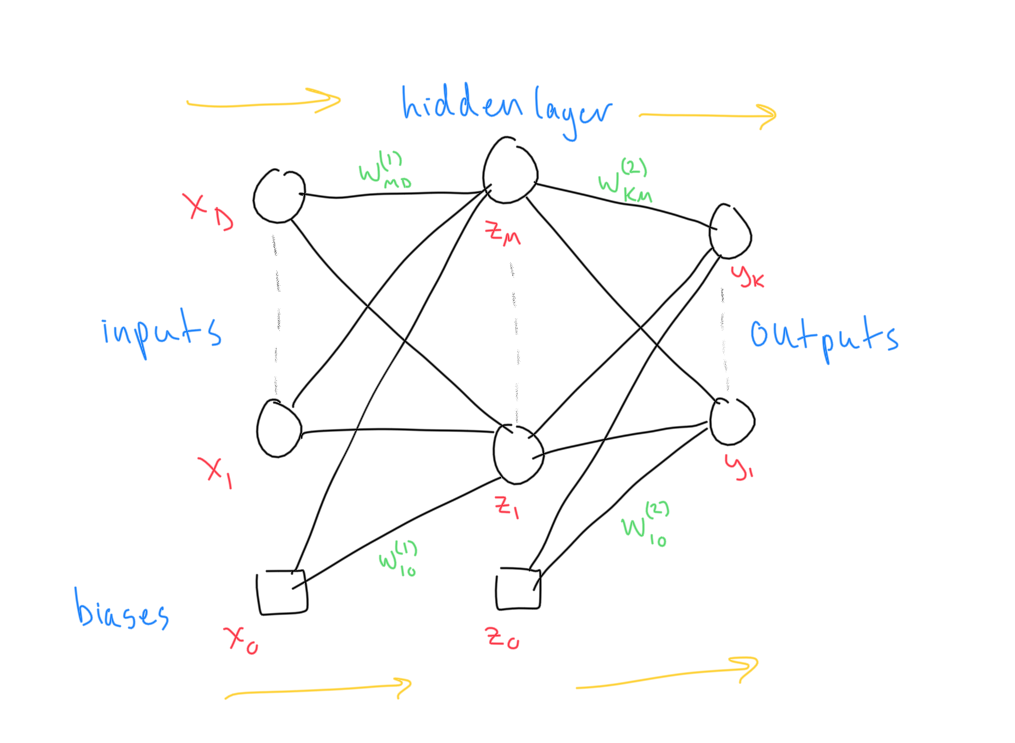
\includegraphics[width=0.5\paperwidth]{../NeuralNetworks/fig/feed-forward-nn.png}
    \caption{Feed Forward Neural Network.}
    \label{fig:feed-foward-nn}
\end{figure}

\readernote{Different resources choose to count the number of layers in a neural net in different manners. We've elected to count each layer of non-input nodes, thus the two-layer network in Figure \ref{fig:feed-foward-nn}. However, some resources will choose to count every layer of nodes (three in this case) and still others count only the number of hidden layers (making this a one hidden layer network).}

Combining Figure \ref{fig:feed-foward-nn} and our preceeding functional description, we can describe the operation performed by a two-layer neural network using a single functional transformation:
\begin{equation} \label{full-nn-equation}
	y_{k}(\textbf{x}, \textbf{w}) = \sigma\bigg(\sum_{m=1}^{M}w_{km}^{(2)} h\bigg(\sum_{d=1}^{D}w_{md}^{(1)}x_{d} + w_{m0}^{(1)}\bigg) + w_{k0}^{(2)}\bigg)
\end{equation}
where we've elected to make the final activation function the sigmoidal function $\sigma(\cdot)$ as we have a binary output activation layer.

Notice that when written like this, a neural network is simply a non-linear function that transforms an input $\textbf{x}$ into an output $\textbf{y}$ that is controlled by our set of parameters $\textbf{w}$.

Furthermore, it may be clear by now why this basic variety of neural networks is referred to as a \textit{feed forward neural network}. If you examine Figure \ref{fig:feed-foward-nn} or Equation \ref{full-nn-equation}, you'll notice that we're simply feeding our input \textbf{x} forward through the network from the first layer to the last layer, hence the name. Assuming we have a fully trained network, we can make predictions on new input data points by propagating them through the network to generate output predictions.

Note that we can also simplify this equation by utilizing the bias trick and appending an $x_{0}=1$ value to each of our data points such that:
\begin{equation*}
	y_{k}(\textbf{x}, \textbf{w}) = \sigma\bigg(\sum_{m=1}^{M}w_{km}^{(2)} h\bigg(\sum_{d=1}^{D}w_{md}^{(1)}x_{d}\bigg)\bigg)
\end{equation*}

Finally, it's worth considering that while a neural network is a series of linear combinations, it is special because of the differentiable non-linearities applied at each of the hidden layers. Without these non-linearities, the successive application of different network weights would be equivalent to a single large linear combination.

Now that we understand the basic structure of a neural network, the important question of how to train our network remains. This is the topic we turn to next.

\section{Network Training}
Now that we understand the structure of a basic feed forward neural network and how they can be used to make predictions, we turn our attention to the training process.

\subsection{Objective Function}
To train our network, it's first necessary to establish a logical objective function for our parameters \textbf{w} that we will seek to minimize. Remember that neural networks can be used to solve both regression and classification problems, which means that our choice of objective will be very much dependent on the type of problem we are working on as well as the properties we desire from that function.

As we've already discussed, for the case of linear regression, a common objective function (but certainly not the only possible one) is the least squares loss function:
\begin{equation} \label{least-squares-loss-function}
	E(\textbf{w}) = \frac{1}{2} \sum_{n=1}^{N} \bigg(y(\textbf{x}_{n}, \textbf{w}) - \textbf{t}_{n}\bigg)^{2}
\end{equation}
For a binary classification problem, which we can model using a sigmoidal nonlinearity in our output activation unit, we'll often use the cross-entropy loss function given by:
\begin{equation} \label{cross-entropy-loss-function}
	E(\textbf{w}) = - \sum_{n=1}^{N} \bigg(y_{n}\ln{\hat{y}_{n}} + (1 - y_{n})(\ln{(1 - \hat{y}_{n})}\bigg)
\end{equation}
And finally, in the multiclass classification setting produced by a softmax function in our output activation layer, we use the following generalizaton to the cross entropy loss function:
\begin{equation} \label{multiclass-cross-entropy-loss-function}
	E(\textbf{w}) = - \sum_{n=1}^{N} \sum_{k=1}^{K} y_{kn} \ln{\bigg(\frac{\text{exp}(a_{k}(\textbf{x}, \textbf{w}))}{\sum_{j=1}^{K}\text{exp}(a_{j}(\textbf{x}, \textbf{w}))}\bigg)}
\end{equation}

\readernote{Loss function, objective function, and cost function all refer to the same concept: the function we optimize to train our model.}

\subsection{Optimizing Parameters}
Ultimately, as we've seen in the preceding two chapters, it is our goal to select a value for our model's weight parameters \textbf{w} that minimizes our objective function. Remember that we did this previously by taking the derivative of our objective with respect to our weight paramters, setting that expression equal to 0, and solving for \textbf{w}. We were previously able to perform that procedure with confidence since we had a convex weight space, which meant the point of minimization for the objective function would occur where $\nabla E(\textbf{w}) = 0$.

Unfortunately for neural networks, this procedure will no longer work quite as well. The objective function, which is parameterized by the weight space, will now have a nonlinear dependence on the weight parameters as a result of the nonlinearities applied to the data points as they are pushed forward through our network. The result of this is that there will be many locations in the parameter space at which the gradient disappears, corresponding to local minima, maxima, or saddle points. This means that we no longer have an analytical solution, and will instead need to resort to a numerical procedure.

\readernote{The terms \textit{analytical} and \textit{numerical} procedures come up very frequently in machine learning literature. An analytical solution typically utilizes a closed form equation that accepts your model and input data and returns a solution in the form of optimized model parameters. On the other hand, numerical solutions are those that require some sort of iteration to move toward an ever better solution, eventually stopping once the solution is deemed `good enough'. Analytical solutions are typically more desirable than numerical solutions due to computational efficiency and performance guarantees, but they often are not possible for complex problems.}

Most numerical techniques utilize some form of gradient based update as follows:
\begin{equation} \label{generic-numerical-update}
	\textbf{w}^{(t+1)} = \textbf{w}^{(t)} + \nabla \textbf{w}^{(t)}
\end{equation}
where $\textbf{w}^{(t)}$ corresponds to the state of the parameters $\textbf{w}$ at time $t$. The parameter values at time $t=0$ given by $\textbf{w}^{(0)}$ are often initialized randomly, and the updates to the parameters $\nabla\textbf{w}^{(t)}$ are computed based on the optimization algorithm being used.

\subsection{Gradient Descent}
We know we need to use a numerical optimization technique to compute our weight parameters $\textbf{w}$, and we've specified a generic form of iterative updates to our weight parameters in Equation \ref{generic-numerical-update}. We will now turn to one of the most common procedures for generating the update $\nabla\textbf{w}^{(t)}$, which is known as gradient descent.

\begin{definition}{Gradient Descent}{gradient-descent}
Gradient descent is a numerical, iterative optimization technique for finding the minimum of a function. It is often used to fit complex model parameters.
\end{definition}

The high level idea behind gradient descent is as follows: to update our parameters, we take a small step in the opposite direction of the gradient of our objective function with respect to the weight parameters $\textbf{w}^{(t)}$. Notationally, this looks like the following:
\begin{equation} \label{gradient-descent-equation}
	\textbf{w}^{(t+1)} = \textbf{w}^{(t)} - \eta \nabla E(\textbf{w}^{(t)})
\end{equation}
where $\eta > 0$ is known as the \textit{learning rate}.

\readernote{In general, we want a learning rate that is large enough so that we make progress toward reaching a better solution, but not so large that we take a step that puts us in a worse place in the parameter space than we were at the previous step. Notice in Figure \ref{fig:gradient-descent-step-size} that an appropriately small step size improves our objective function, while a large step size overshoots the update and leaves us in a worse position.}

\begin{figure}
    \centering
    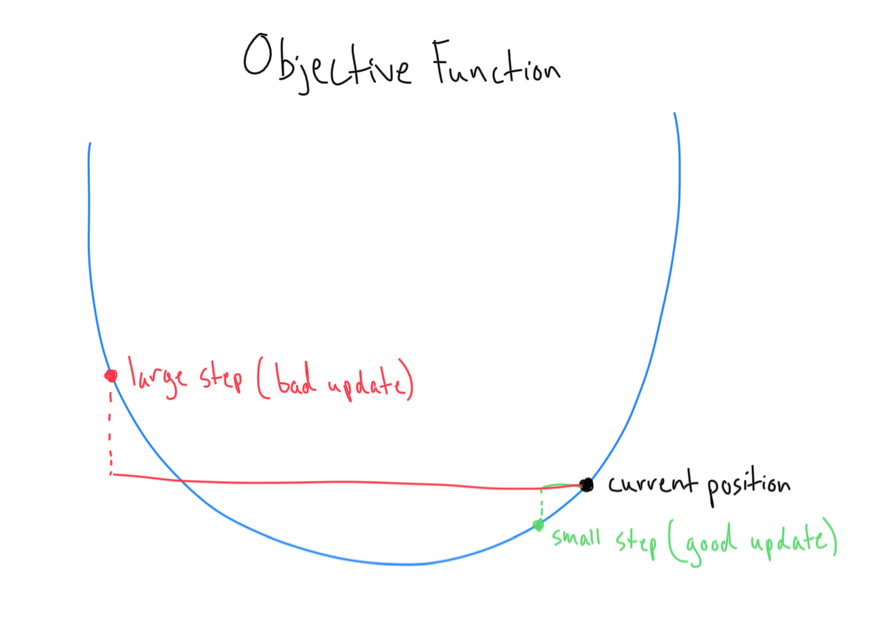
\includegraphics[width=0.5\paperwidth]{../NeuralNetworks/fig/objective-function-nn.png}
    \caption{Step Size in Gradient Descent.}
    \label{fig:gradient-descent-step-size}
\end{figure}

Why take a step in the opposite direction of the gradient of the objective function? You can think of the objective function as a hill, and the current state of our parameters $\textbf{w}^{(t)}$ is our position on that hill. The gradient tells us the steepest direction of increase in the objective function (i.e. it specifies the direction that will make our model worse). Since we want to minimize the objective function, we choose to move away from the direction of the gradient, sending our model down the hill towards an area of lower error. We typically cease optimization when our updates become sufficiently small, indicating that we've reached a local minimum. Note that it's a good idea to run gradient descent multiple times to settle on a final value for $\textbf{w}$, ideally initializing $\textbf{w}^{(0)}$ to a different starting value each time, because we are optimizing a function with multiple local minima.

There are different means by which we can compute the gradient of our objective function at each step. The first way, often called \textit{batch gradient descent}, computes the gradient for our objective function at each step using the entire data set. In contrast, the technique known as \textit{stochastic gradient descent} (also known as SGD) utilzies a subset of the data points at each step to compute the gradient, sometimes just one. Stochastic gradient descent is typically a more popular technique for several reasons. First, the computation time is often significantly smaller as you don't need to pass over the entire data set at each iteration. Furthermore, it's less likely that you will get stuck in local minima while running SGD because a point in the parameter space that is a local minima for the entire data set combined is much less likely to be a local minima for each data point individually. Finally, SGD lends itself to being used for training online models (meaning models built on data points that are arriving at regular intervals) as the entirety of the data does not need to be present in order to train.

\subsection{Backpropagation}
While we've explained at a high level how we use gradient descent to find a good setting for our weight parameters $\textbf{w}$, we have not discussed how we compute the gradient of our objective function with respect to our weights. Thinking again about how our feed forward neural network works, by propagating activations through our network to produce a final output, it's not immediately clear how we can compute gradients for the weights that lie in the middle of our network, as we don't actually have expected results for those intermediate values. The solution to this problem is to send errors backwards through our network in a process known as \textit{backpropagation}.

\begin{definition}{Backpropagation}{backpropagation}
Backpropagation is the procedure by which we pass errors backwards through a feed forward neural network in order to compute gradients for the weight parameters of the network.
\end{definition}

Backpropagation refers specifically to the portion of neural network training during which we compute the derivative of the objective function with respect to the weight parameters. This is done by propagating errors backwards through the network, hence the name.

\readernote{Note that we still need to update the value of the weight parameters after computing their derivatives. This is typically done using gradient descent or some variant of it.}

We now explore the details of backpropagation in greater depth.

\subsection{Computing Derivatives Using Backpropagation}
Recall that the activation $a_{j}$ for an arbitrary node in a neural network can be described by the equation:
\begin{equation} \label{activations-reminder}
	a_{j} = \sum_{m=1}^{M} w_{jm} z_{m}
\end{equation}
where there are $M$ incoming nodes $z_{1}, ..., z_{M}$ connected to the node of interest and weighted by $w_{j1}, ..., w_{jM}$ as we see in Equation \ref{basic-nn-form-next-layer} and Figure \ref{fig:feed-foward-nn}. Recall also that this sum is then transformed by an arbitrary activation function $h(\cdot)$ (which is typically nonlinear) to give the activation $z_{j}$:
\begin{equation} \label{transformed-activations-reminder}
	z_{j} = h(a_{j})
\end{equation}
computing these values as we flow through the network constitutes the forward pass through our network.

We now wish to begin the process of computing derivatives of the objective function with respect to our weights. For the sake of simplicity, we'll assume that the current setting of our parameters $\textbf{w}$ generates an error of $E$ for a single data point, as though we were performing stochastic gradient descent.

Let's consider how we could compute the derivative of $E$ with respect to an individual weight in our network, $w_{jm}$:
\begin{equation} \label{deriv-E-wrt-wjm}
	\frac{\partial E}{\partial w_{jm}}
\end{equation}
We first need to figure out what the dependence of $E$ is on this single weight $w_{jm}$. This weight contributes to the final result only via its contribution to the activation $a_{j}$. This allows us to use the chain rule to simplify Equation \ref{deriv-E-wrt-wjm} as:
\begin{equation} \label{chain-rule-deriv-E-wrt-wjm}
	\frac{\partial E}{\partial w_{jm}} = \frac{\partial E}{\partial a_{j}} \cdot \frac{\partial a_{j}}{\partial w_{jm}}
\end{equation}
Using Equation \ref{activations-reminder}, we have that:
\begin{equation*}
	\frac{\partial a_{j}}{\partial w_{jm}} = z_{m}
\end{equation*}
We now introduce the following notation for the sake of simplicity:
\begin{equation} \label{delta-expression}
	\delta_{j} = \frac{\partial E}{\partial a_{j}}
\end{equation}
where the values of $\delta_{j}$ are referred to as \textit{errors}. Now, we are able to rewrite Equation \ref{chain-rule-deriv-E-wrt-wjm} as:
\begin{equation} \label{simplified-chain-rule-deriv-E-wrt-wjm}
	\frac{\partial E}{\partial w_{jm}} = \delta_{j} z_{m}
\end{equation}

The implications of Equation \ref{simplified-chain-rule-deriv-E-wrt-wjm} are significant for understanding backpropagation. It indicates that the derivative of the objective function with respect to an arbitrary weight in the network is equal to the product of the error $\delta$ at the output end of that weight and the value $z$ at the input end of the weight. We can visualize this property in Figure \ref{fig:backprop-gradient}.

\begin{figure}
    \centering
    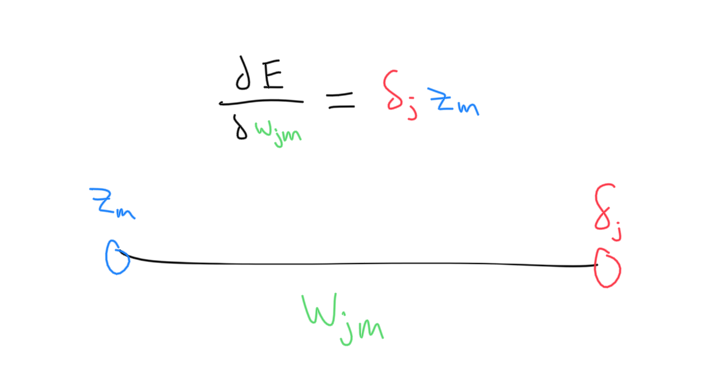
\includegraphics[width=0.5\paperwidth]{../NeuralNetworks/fig/backprop-gradient.png}
    \caption{Gradient of the objective function with respect to a weight.}
    \label{fig:backprop-gradient}
\end{figure}

Thus, to compute all the derivatives of the network, we need only to compute the values of $\delta_{j}$ for each of the nodes in the network. The values of $z_{m}$ should be saved during the forward pass through the network to be multiplied by the values of $\delta_{j}$.
\readernote{We will only have errors $\delta_{j}$ for the hidden and output units of our network. This is logical because there is no notion of applying an error to our input data, which we have no control over.}
We now need only to consider how we should compute the values of $\delta_{j}$, given by Equation \ref{delta-expression}.
For the final layer, also called the output layer, the error is simply the difference between what we computed by propagating the input through the network and the known result:
\begin{equation*}
	\delta_{j} = \hat{y}_{k} - y_{k}
\end{equation*}
We've seen this term, the difference between the expected and actual results, arise in the gradient of our error expressions for both linear regression and classification in the previous two chapters.

To compute the errors $\delta_{j}$ for the hidden units, we again make use of the chain rule to decompose the errors $\delta_{j}$ as follows:
\begin{equation} \label{backprop-for-deltas}
	\delta_{j} = \frac{\partial E}{\partial a_{j}} = \sum_{m=1}^{M} \frac{\partial E}{\partial a_{m}} \frac{\partial a_{m}}{\partial a_{j}} 
\end{equation}
where the summation runs over all of the $M$ nodes to which the node $j$ sends connections as seen in Figure \ref{fig:sum-over-nodes}.

\begin{figure}
    \centering
    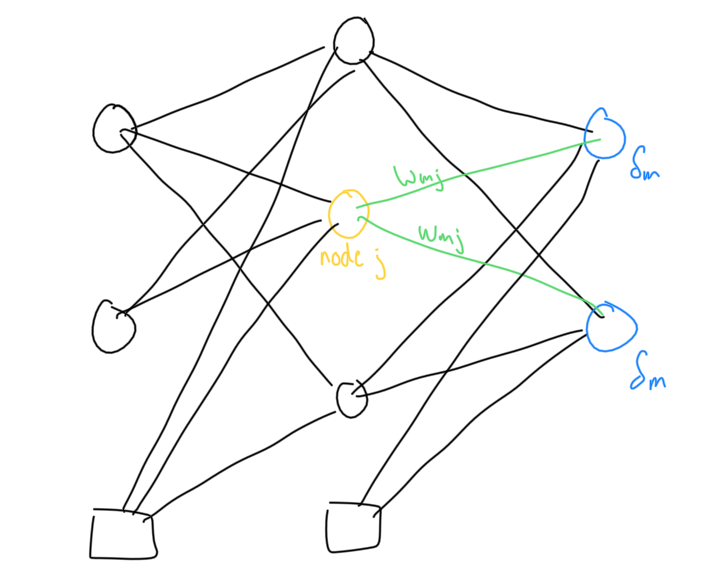
\includegraphics[width=0.5\paperwidth]{../NeuralNetworks/fig/sum-over-nodes.png}
    \caption{Summation over the nodes (blue) to which node j (gold) sends connections (green).}
    \label{fig:sum-over-nodes}
\end{figure}

We can rewrite this expression using Equations \ref{delta-expression}, \ref{activations-reminder}, and \ref{transformed-activations-reminder}:
\begin{equation} \label{backprop-formula}
	\delta_{j} = h'(a_{j}) \sum_{m=1}^{M} w_{mj} \delta_{m}
\end{equation}
which means that the value of $\delta$ for a given node can be computed by passing back (backpropagating) the errors $\delta$ from nodes farther up in the network!

Since we know the values of $\delta$ for the final layer of output node, we can recursively apply Equation \ref{backprop-formula} to compute the values of $\delta$ for all the nodes in the network.

Remember that all of these calculations were done for a single input data point that generated the error $E$. If we were using stochastic gradient descent, we would perform the same calculation for each data point in our mini-batch, and then sum the gradients as follows:

\begin{equation} \label{batch-errors-backprop}
	\frac{\partial E}{\partial w_{jm}} = \sum_{n=1}^{N} \frac{\partial E_{n}}{\partial w_{jm}}
\end{equation}

To solidify our understanding of the backpropagation algorithm, it can be useful to try a concrete example.

\begin{example}{Backpropagation Example}{backprop-example}
	Imagine the case of a simple two layer neural network as in Figure \ref{fig:feed-foward-nn}. We'll use the standard quadratic loss function on our output layer:
	\begin{align*}
		E = \frac{1}{2} \sum_{m=1}^{M} (\hat{y}_{m} - y_{m})^{2}
	\end{align*}
	Where $M$ is the number of units in the output layer. To the hidden units, we'll apply a nonlinear sigmoidal activation function given by:
	\begin{align*}
		\sigma(z) = \frac{1}{1 + \exp{(-z)}}
	\end{align*}
	whose derivative is given by:
	\begin{align*}
		\frac{\partial \sigma(z)}{\partial z} = \sigma(z)(1 - \sigma(z))
	\end{align*}
	For our input data point $\textbf{x}$, we forward propagate through our network to get the activations of the hidden layer:
	\begin{align*}
		a_{j} = \sum_{d=0}^{D} w_{jd}^{(1)} x_{d}
	\end{align*}
	We then transform this value using our sigmoidal nonlinearity:
	\begin{align*}
		z_{j} = \sigma{(a_{j})}
	\end{align*}
	We then propagate these transformed activations forward once more to get our output activations:
	\begin{align*}
		\hat{y}_{m} = \sum_{j=0}^{J} w_{mj}^{(2)} z_{j}
	\end{align*}
	Now that we've propagated forward, we can begin to propagate our errors backwards! We start by computing the errors for the output layer as follows:
	\begin{align*}
		\delta_{m} = \hat{y}_{m} - y_{m}
	\end{align*}
	We then backpropagate these errors back to the hidden units as follows:
	\begin{align*}
		\delta_{j} = (\sigma(z_{j})(1 - \sigma(z_{j}))) \sum_{m=1}^{M} w_{mj} \delta_{m}
	\end{align*}
	And now that we have our errors for the hidden and output layers, we can compute the derivative of the loss with respect to our weights as follows:
	\begin{align*}
		\frac{\partial E}{\partial w_{jd}^{(1)}} = \delta_{j} x_{d}, \quad \frac{\partial E}{\partial w_{mj}^{(2)}} = \delta_{m} z_{j}
	\end{align*}
	We then use these derivatives along wtih an optimization technique such as gradient descent to improve our model weights.
\end{example}

\section{Choosing a Network Structure}
Now that we know the general form of a neural network and how the training process works, we must step back and consider the question of how we actually arrive at an optimal network structure. We'll begin with an idea we've already seen before: cross validation.

\subsection{Cross Validation for Neural Networks}
We've previously discussed cross validation in the chapter on linear regression. We used it then to compare the performance of different models, attempting to identify the best model while also avoiding overfitting. We can use a similar process to identify a reasonable network structure.

First of all, the input and output parameters of a neural network are generally decided for us: the dimensionality of our input data dictates the number of input units and the dimensionality of the required output dictates the number of output units. For example, if we have an 8-by-8 pixel image and need to predict whether it is a `0' or a `1', our input dimensions are fixed at 64 and our output dimensions are fixed at 2. Depending on whether you wish to perform some sort of pre or post-processing on the inputs/outputs of your network, this might not actually be the case, but in general when choosing a network structure we don't consider the first or last layer of nodes as being a relevant knob that we can tune.

That leaves us to choose the structure of the hidden layers in our network. To make this problem more tractable, we can simplify it even further: we'll consider the total number of units contained in our hidden layers (meaning we sum the units from each hidden layer). So if we have three hidden layers each with 5 units each, we'll have 15 total units for that network structure.

Unsurprisingly, the more hidden units we have for our model, the more variation we will produce in our results and the closer we will come to overfitting.

Thus, we can use cross validation in the same way we've done before: train our model with differing numbers of internal units and structures (as in Figure \ref{fig:internal-node-differences}) and then select the model that performs best on the validation set.

\begin{figure}
    \centering
    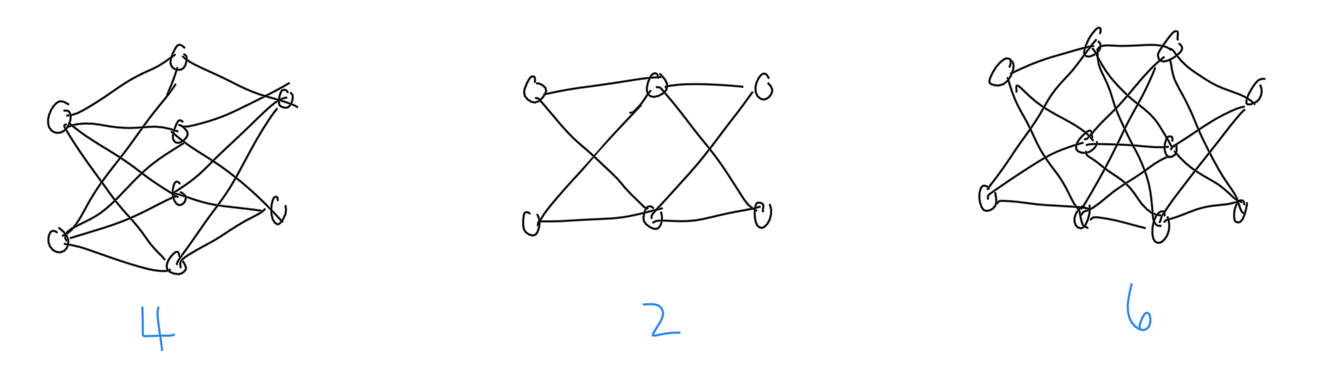
\includegraphics[width=0.5\paperwidth]{../NeuralNetworks/fig/internal-node-differences.png}
    \caption{Networks with different structures and numbers of internal nodes.}
    \label{fig:internal-node-differences}
\end{figure}

\readernote{There are other considerations at play beyond performance when choosing a network structure. For example, the more internal units you have in your network, the more storage and compute time you will need to train them. If either training time or response time after training a model is critical, you may need to consider consolidating your network at the expense of some performace.}

\subsection{Regularization}
You can also apply regularization to the weights in your network to help prevent overfitting. For example, we could introduce a simple quadratic regularizer of the form $\frac{\lambda}{2} \textbf{w}^{T}\textbf{w}$ to our objective function. There are other considerations to be made here, for example we would like our regularizer to be invariant to scaling, meaning that multiplying our input data by a constant would produce a proportionally equivalent network after training. The quadratic regularizer is not invariant to scaling, but the basic concept of avoiding extreme weights is the same nonetheless.

\subsection{Data Augmentation}
We can use transformations to augment our data sets, which helps prevent overfitting. This technique is not specific to neural networks, but often the types of unstructured data for which we use neural networks can benefit greatly from it.
\begin{definition}{Data Augmentation}{data-augmentation}
Data augmentation refers to the practice of increasing the size and diversity of your training data by applying transformations to the initial data set.
\end{definition}
For example, if we are working with image data, we might choose to rotate or reflect the image, depending on the type of network we are trying to build and whether or not this would preserve the integrity of the image. We might also change something like the brightness or density of the image data. In this way, we can produce more and more varied training points, thus reducing the likelihood of overfitting.

\section{Specialized Forms of Neural Networks}
Simple neural networks are useful for a general set of tasks, and as universal function approximators, they \textit{could} be useful for any task. However, there are certain data types and use cases for which we've developed more specialized forms of neural networks that perform even better in their respective domains. We will take a high level view of these different flavors of neural networks.

\subsection{Convolutional Neural Networks (CNNs)}
Convolutional neural networks (abbreviated CNNs) are most often used for image data, but their underlying principles apply in other domains as well.

To understand why a CNN is useful, consider this specific problem: you are trying to determine whether or not there is a dog in an image. There are two general difficulties we have to deal with in solving this problem. First, while dogs have a lot of similar features (ears, tails, paws, etc.), we need some means of breaking an image down into smaller pieces that we can identify as being ears or tails or paws. Second, what happens if we train on images of dogs that are all in the center of the photo, and then we try to test our network on an image where the dog is in the upper left hand corner? It's going to fail miserably.

CNNs overcome these problems by extracting smaller local features from images via what's known as a \textit{sliding window}. You can imagine this sliding window as a matrix kernel that moves over every subsection of an image, producing a summary of those subsections that feed into the next layer in our network. We do this over the entire image, and with several different sliding windows. Without going into too many details, this solves the two general problems we had above: our small sliding window can summarize a feature of interest (such as a dog ear) and it is also location invariant, meaning that we can identify that dog ear anywhere in an image.

\begin{figure}
    \centering
    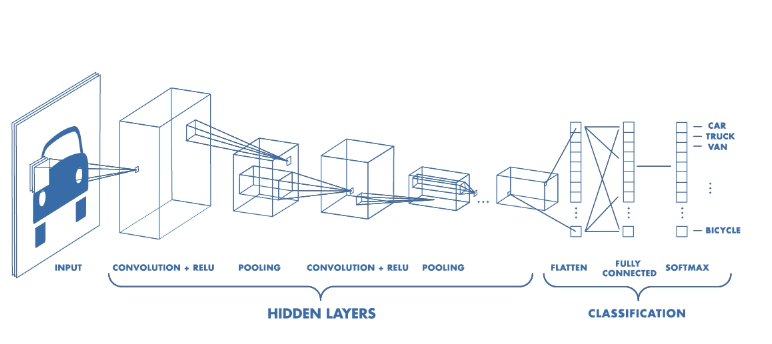
\includegraphics[width=0.5\paperwidth]{../NeuralNetworks/fig/CNN-structure.png}
    \caption{Excellent diagram of the structure of a CNN. source: https://www.mathworks.com/videos/introduction-to-deep-learning-what-are-convolutional-neural-networks--1489512765771.html}
    \label{fig:CNN-structre}
\end{figure}

\subsection{Recurrent Neural Networks (RNNs)}
As with CNNs, recurrent neural networks (abbreviated RNNs) are used to more efficiently solve a specific problem type. To motivate the structure of an RNN, we will turn again to a specific example.

Imagine we were building a tool with the goal of predicting what word comes next in a newspaper article. Obviously, the words that came before the word that we are currently trying to predict are crucial to predicting the next word. Imagine we propagate the preceding ten words through our network to predict which word we think will come next. It would also be useful if we could send some of the information at each layer backwards through the network to help with the next prediction - since we know the sequence of words matters. In this sense, our network is `stateful' because it's remembering what came before. We don't have this ability with a feed-forward network, which by design only propagates information forward through the network. RNNs add backward passing of activations into their network structure to improve predictions on data where there is some temporal dependence on what came previously.

\begin{figure}
    \centering
    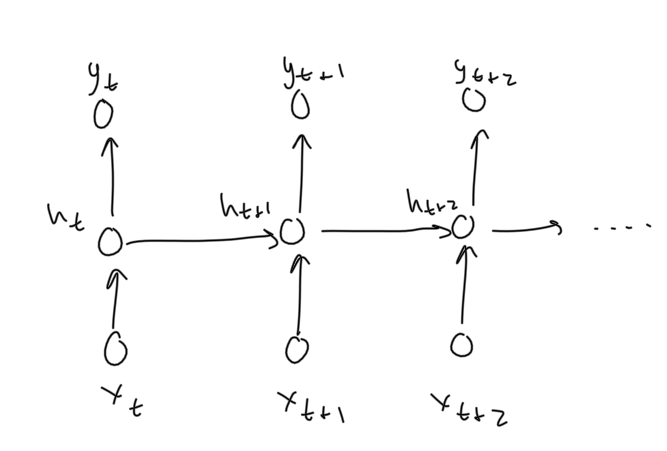
\includegraphics[width=0.5\paperwidth]{../NeuralNetworks/fig/RNN-structure.png}
    \caption{Simple example of an RNN. The blue connections pass activations backwards.}
    \label{fig:RNN-structre}
\end{figure}


\subsection{Bayesian Neural Networks (BNNs)}
Up until now, our training process has been one of maximum likelihood estimation, or a maximum posterior approach if we utilize a regularizer that can be interpreted as introducing a prior.

A Bayesian neural network, or BNN, does exactly what you might imagine: it introduces a distribution over the parameters of our model, which then requires marginalizing over those distributions in order to make a prediction. The specifics of how exactly a BNN is constructed are beyond the scope of this textbook, but the idea behind why we would utilize a BNN is the same as the reason we utilize Bayesian techniques in other domains, particularly the use of prior information to aid model performance.